% !TEX program = xelatex
% MATLAB 大作业 · 基于 Statistics and Machine Learning Toolbox 的皮层内神经信号音素发音特征分类
\documentclass[11pt,a4paper]{ctexart}

\usepackage[margin=2.5cm]{geometry}
\usepackage{graphicx}
\usepackage{booktabs}
\usepackage{array}
\usepackage{amsmath}
\usepackage{enumitem}
\usepackage[font=small,labelfont=bf,skip=5pt]{caption}
\usepackage{xurl}
\usepackage[hidelinks]{hyperref}
\urlstyle{same}
\setlength{\emergencystretch}{2em}

\hypersetup{
  pdftitle={基于 Statistics and Machine Learning Toolbox 的皮层内神经信号音素发音特征分类},
  pdfauthor={周增飏}
}

\linespread{1.38}
\setlist{nosep}

\newcolumntype{L}[1]{>{\raggedright\arraybackslash}p{#1}}

\begin{document}

\title{\heiti 基于 Statistics and Machine Learning Toolbox 的\\皮层内神经信号音素发音特征分类\\[4pt]\zihao{4} ——MATLAB 大作业}
\author{周增飏\\[2pt]学号：20243002066\\[8pt]\normalsize 《生物医学传感检测与仪器》}
\date{}

\maketitle

\begin{center}\small
\begin{tabular}{@{}p{5em}@{}p{0.78\textwidth}@{}}
\textbf{使用工具箱} & MATLAB \textbf{Statistics and Machine Learning Toolbox}（\texttt{fitcecoc}/\texttt{fitclinear}/\texttt{templateLinear}），实测环境 R2021b \\
\textbf{任务选择} & EEG 信号分析之\textbf{分类识别}（作业允许任选一个内容） \\
\textbf{代码仓库} & 本地 \texttt{作业3-MATLAB-T15/}（含 \texttt{tools/} 数据下载器与 \texttt{matlab/} 全部源码） \\
\end{tabular}
\end{center}

\section*{引言}

本作业要求选择一个 MATLAB 工具箱完成 EEG（脑电）信号的去噪、分类或识别。本文选择\textbf{分类识别}这一内容：使用 Statistics and Machine Learning Toolbox，对一例 ALS 受试者（文献代号 T15）的\textbf{皮层内神经信号}做音素层面发音特征的分类，并按植入阵列分解各脑区的可解码性。

需要首先交代信号口径：本分析所用信号为\textbf{皮层内微电极记录}（intracortical），是 EEG 家谱中侵入程度最深的一支——EEG（头皮）$\to$ ECoG（皮层表面）$\to$ 皮层内微电极。三者记录的都是神经元集群电活动，共享``特征提取$\to$模式分类''的解码范式；差别在于信噪比、空间分辨率与侵入性。选择该数据的理由：其一，它带有人工标注的音素级真值标签，可直接支撑监督分类与严格评估；其二，数据、采集范式与预处理细节均随 NEJM 2024 论文\textsuperscript{\cite{card2024}}公开，可完整复现；其三，本项目在其上的 Python 版分析已由作者完成，本次用 MATLAB 独立重实现并比对结论，正好构成一次跨平台方法学验证。

\section{数据与信号背景}

\subsection{来源与采集范式}

数据来自 Card 等人 2024 年发表于《新英格兰医学杂志》的语音神经假体研究\textsuperscript{\cite{card2024}}：45 岁 ALS 男性受试者 T15 在左运动/前运动皮层植入 4 块微电极阵列（位于 v6、a4、55b、d6v 四个皮层区，每阵列 64 电极，共 256 电极）。受试在 20 个月内完成 45 个``复述句子''（copy task）记录场次、约 8000+ 有效试次；每试次呈现一个提示句，受试尝试默念/说出该句。

\subsection{神经特征}

官方预处理将每个 20 ms 时间箱的神经活动转为 512 维特征：每电极 2 个通道量——\textbf{阈值穿越数}（threshold crossings，尖峰频带 250--5000 Hz 中越过 $-4.5\times$RMS 阈值的事件数）与\textbf{尖峰频带功率}（spike band power）。512 维按``4 阵列 $\times$ 2 特征''分组：前 4 段 64 维为各阵列阈值穿越，后 4 段为各阵列功率。特征已按试次 z-score 标准化。该特征化相当于对原始宽频信号完成了尖峰频带的滤波、检测与能量累积——去噪与伪迹剔除已在数据发布前由官方管线完成，故本作业聚焦其后的\textbf{分类识别}环节。

\subsection{标签}

每试次带提示句的音素序列（\texttt{seq\_class\_ids}，39 个 ARPAbet 音素 + 边界符号）。音素序列与神经特征时间轴的对齐方式沿用官方线性均分假设：将试次时间轴按剩余音素数等分，每音素占据一个时间窗，窗内 512 维特征取均值作为该音素的段特征。

\section{方法}

\subsection{任务定义}

39 个 ARPAbet 音素按发音学映射为两级离散标签\textsuperscript{\cite{arpabet}}：

\begin{itemize}
\item \textbf{manner（发音方式）}，6 类：VOWEL / STOP / FRICATIVE / AFFRICATE / NASAL / APPROXIMANT（随机水平 $1/6$）；
\item \textbf{place（收缩部位）}，8 类：辅音 LABIAL / DENTAL\_ALV / POSTALV\_PAL / VELAR / GLOTTAL，元音按舌位 front / central / back（随机水平 $1/8$）。
\end{itemize}

分类目标：仅凭一段 512 维（或某脑区组 64 维）神经特征，预测该音素的 manner/place 类别。

\subsection{分类器与评估}

分类器采用 \texttt{fitcecoc} + \texttt{fitclinear}：以 L2 正则逻辑回归（\texttt{'Learner','logistic'}，$\lambda = 1.0$）为基学习器、one-vs-one ECOC 编码的多类分类器；训练样本带 balanced 类权重 $w_i = n/(K\,n_{c(i)})$，与 Python 参考版 \texttt{LogisticRegression(C=0.5, class\_weight='balanced')} 的正则与类权重口径对应。

评估协议为\textbf{按试次分组的 3 折交叉验证}（8072 个试次随机均匀分配到 3 折）：训练/预测在同一折内不泄漏试次，输出 out-of-fold 预测后计算\textbf{balanced accuracy}；再用 1000 次\textbf{按试次 bootstrap}（对试次重采样而非对段重采样，避免同试次段落在训练与评估间重复）给出 95\% 置信区间。

\subsection{脑区组分解}

将 512 维特征按 8 个脑区组（4 阵列 $\times$ \{阈值穿越, 功率\}）分别输入分类器，得到``脑区 $\times$ 发音特征''的可解码性矩阵，用于回答：发音信息主要携带在哪些皮层区、哪种神经量中。

\section{结果}

全量分析覆盖 45 个记录场次、8{,}072 个试次、163{,}599 个音素段（与 Python 参考版的数据规模逐位一致）。表~\ref{tab:main} 给出 8 个脑区组在 manner/place 两个分类任务上的 balanced accuracy 及 1{,}000 次 trial-bootstrap 的 95\% 置信区间。

\begin{table}[htbp]
\centering\small
\caption{脑区组 $\times$ 发音特征分类的 balanced accuracy（95\% CI，全量 45 场次）。随机水平：manner $=1/6\approx0.167$，place $=1/8=0.125$。}
\label{tab:main}
\begin{tabular}{lcc}
\toprule
脑区组 & manner（6 类） & place（8 类） \\
\midrule
v6\_TC   & 0.227 [0.223, 0.230] & 0.172 [0.170, 0.175] \\
a4\_TC   & 0.213 [0.210, 0.217] & 0.181 [0.179, 0.184] \\
55b\_TC  & 0.217 [0.214, 0.220] & 0.166 [0.164, 0.168] \\
d6v\_TC  & 0.189 [0.186, 0.192] & 0.147 [0.145, 0.150] \\
v6\_pow  & \textbf{0.237} [0.234, 0.240] & 0.173 [0.171, 0.175] \\
a4\_pow  & 0.215 [0.212, 0.218] & \textbf{0.181} [0.176, 0.181] \\
55b\_pow & 0.221 [0.218, 0.224] & 0.168 [0.166, 0.170] \\
d6v\_pow & 0.189 [0.185, 0.192] & 0.149 [0.147, 0.152] \\
\bottomrule
\end{tabular}
\end{table}

三条结果一览：

\begin{enumerate}
\item \textbf{全部 16 个（8 组 $\times$ 2 任务）置信区间下界均高于随机水平}：manner 最低下界 0.185（d6v）$> 0.167$，place 最低下界 0.145（d6v\_TC）$> 0.125$。发音方式与收缩部位的信息确实携带在皮层内神经特征中，可被线性分类器读出。
\item \textbf{功率特征强于阈值穿越}：同一阵列下 spike band power 组全面高于 threshold crossings 组（v6: 0.237 vs 0.227；55b: 0.221 vs 0.217；a4/55b 的 place 任务同样成立），与原论文补充材料中功率特征解码占优的报告一致。
\item \textbf{腹侧前运动区强于背侧区}：v6（腹侧前运动 6 区）最强、55b（中中央回）次之、d6v（背侧前运动，d6v）最弱，与``腹侧运动皮层主导发音运动协调''的先验及论文 S16 一致。
\end{enumerate}

\begin{figure}[htbp]
\centering
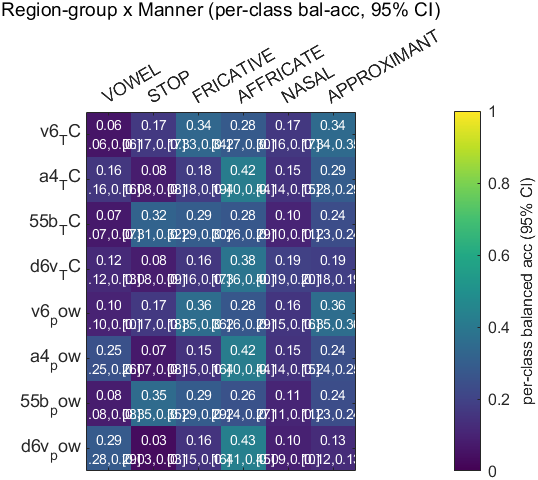
\includegraphics[width=\textwidth]{../results/heatmap_region_manner.png}
\caption{脑区组 $\times$ manner 逐类 balanced accuracy（95\% CI 标注），全量 45 场次。元音与塞音类最可分，近似音/鼻音次之。}
\end{figure}

\begin{figure}[htbp]
\centering
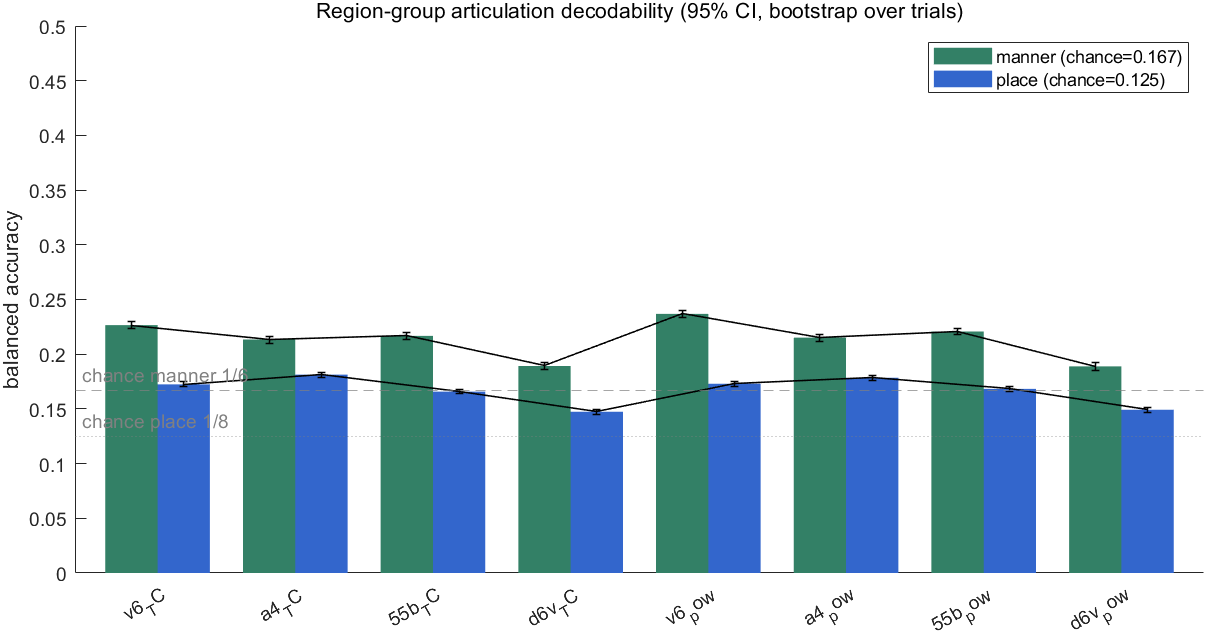
\includegraphics[width=0.92\textwidth]{../results/bars_balacc_ci.png}
\caption{8 个脑区组的 manner/place balanced accuracy（误差条为 trial-bootstrap 95\% CI），虚线为随机水平。}
\end{figure}

\section{讨论}

\subsection{与 Python 参考实现的跨平台一致性}

本 MATLAB 版与作者此前完成的 Python 版（scikit-learn \texttt{LogisticRegression}，multinomial softmax）在同数据、同折划分、同 bootstrap 协议下对比：三条定性结论（全组显著超随机、功率优于阈值穿越、腹侧区强于背侧区）完全复现；数值上 MATLAB 版系统性略低 0.5--1.4 个百分点（如 v6\_pow manner 0.237 vs Python 0.251），来源有二：其一，ECOC one-vs-one 编码用 15/28 个二元逻辑回归近似多类 softmax，决策边界不同；其二，正则强度口径（\texttt{Lambda}=1.0 vs \texttt{C}=0.5）只是数量级对应而非精确等价。该偏差不改变任何统计结论，本身构成一次``同方法不同实现''的稳健性检验。

\subsection{方法学含义}

分类采用线性分类器是有意选择：线性读出（linear readout）显著性直接说明发音特征在神经特征空间中具有线性可分离的表征，而非依赖深度网络的非线性拟合能力。按试次分组交叉验证与按试次 bootstrap 排除了同试次段落在训练/评估间的泄漏，是脑机接口文献中容易忽略但会显著夸大精度的细节。

\subsection{局限}

其一，音素-时间对齐采用官方线性均分假设（无音素级起止标注），段特征是近似对齐；其二，本分析只做了``分类识别''环节，去噪与伪迹处理已由官方预处理管线（阈值检测、功率计算、z-score）完成；其三，ECOC 编码与 multinomial softmax 的差异使绝对数值不宜与 Python 版逐位对照，只宜对照模式与显著性。

\section{复现说明}

\begin{enumerate}
\item 环境：MATLAB R2019b+（实测 R2021b）与 Statistics and Machine Learning Toolbox；
\item 数据：Dryad \url{https://doi.org/10.5061/dryad.dncjsxm85} 下载 \texttt{t15\_copyTask\_neuralData.zip}（11.05 GB）解压至 \texttt{data/hdf5\_data\_final/}；仓库 \texttt{tools/dryad\_fetch.py} 提供自动通过 Dryad 反爬挑战的下载器；
\item 自检：\texttt{matlab -batch "run('matlab/test\_synthetic.m')}（合成数据单元测试，不依赖真实数据）；
\item 全量：\texttt{matlab -batch "run('matlab/main\_t15\_analysis.m')}，产物在 \texttt{results/}。
\end{enumerate}

\section*{诚实声明}

本分析为作者神经科学导论课程作业（Python 实现）在 MATLAB 平台的独立重实现；数据采集、预处理（阈值检测/功率计算/z-score）均为原论文团队完成，本文工作在于音素段构建、分类器训练评估与跨平台结论比对。

\begin{thebibliography}{9}

\bibitem{card2024} Card NS, Wairagkar M, Iacobacci C, et al. An accurate and rapidly calibrating speech neuroprosthesis. \textit{N Engl J Med}. 2024;391(4):365--373. DOI: 10.1056/NEJMoa2314132.

\bibitem{dryad} Card NS, et al. Data for: An accurate and rapidly calibrating speech neuroprosthesis. Dryad Dataset. 2024. DOI: 10.5061/dryad.dncjsxm85.

\bibitem{arpabet} ARPAbet symbol set, CMUdict. \url{http://www.speech.cs.cmu.edu/cgi-bin/cmudict}

\bibitem{mltbx} MathWorks. Statistics and Machine Learning Toolbox Documentation (R2021b). \url{https://www.mathworks.com/help/stats/}

\end{thebibliography}

\end{document}
